% The 'documentclass' controls the overall form of presentation, e.g. resume, article, etc.
% The 'beamer' documentclass creates a document in the appearance of slides.
\documentclass{beamer}
% Functions to be called begin with a '\', e.g. '\documentclass'.
% Main parameters are between braces, e.g. '{beamer}'.
% Additional parameters are a comma-separated list in brackets, e.g. '12pt, letterpaper'.

% This is the 'preamble', it defines general parameters and data that can be utilized later
% by other commands, such as '\titlepage'.
\title{Business.com Pitch Deck}
\author{Vijay,Steven,Mattias,Fillipo}
\institute{Overleaf}
\date{2021}
\logo{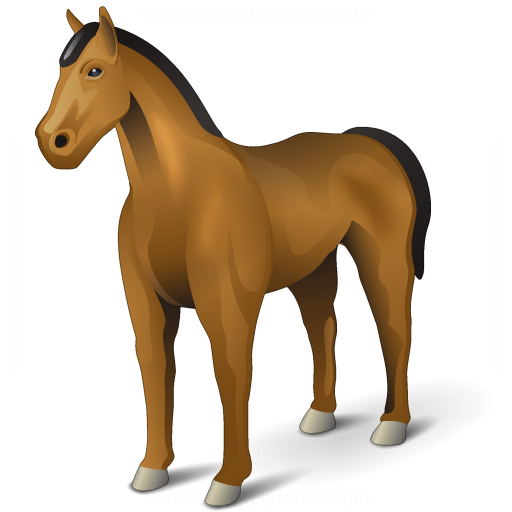
\includegraphics[width=1cm]{HorseIcon.png}}

\usetheme{Madrid}

% Start the main body of the document being created.
\begin{document}

% This is using the normal latex command '\frame', which puts a rectangular frame around the
% contents.
\frame{\titlepage}

\begin{frame}
\frametitle{Sample frame title}
\begin{itemize}
  \item This is some text in the first frame.
  \item This is some text in the first frame.
  \item This is some text in the first frame.
\end{itemize}
\end{frame}


\begin{frame}
\frametitle{A Frame with an Image}
\begin{columns}

\begin{column}{0.5\textwidth}
  \centering
    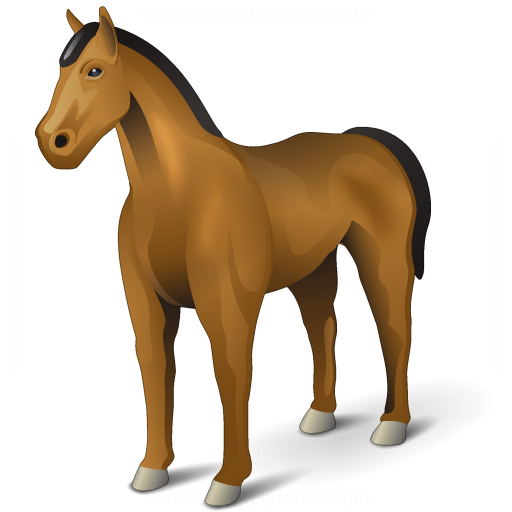
\includegraphics[width=4cm]{HorseIcon.png}
\end{column}

\begin{column}{0.5\textwidth}
\begin{itemize}
  \item Point 1
  \item Point 2
  \item Point 3
\end{itemize}
\end{column}

\end{columns}

\end{frame}

% Finish the main body of the document being created.
\end{document}